\documentclass[12pt]{article}
\usepackage{../lecture}
\lecture{10}{Reductions and Recursion}
\date{March 2, 2021}

\begin{document}
\maketitle

\section{Algorithms}
\begin{itemize}
    \item Formally, an algorithmic problem is the task of computing some function $f: \sum^{\ast} \rightarrow \sum^{\ast}$.
    \item Input $w \in \sum^{\ast}$ is an encoding of a "valid input" and output $w \in \sum^{\ast}$ is also an encoding.
    \item An \textbf{algorithm} is a "program" $A$ such that $\forall w \in \sum^{\ast}, A(w) = f(w)$.
\end{itemize}

\subsection{Turing-Complete Model}
\begin{itemize}
    \item We will assume a unit-cost RAM model:
    \begin{itemize}
        \item The basic data is an integer.
        \item Numbers fit into "words".
        \item Artihmetic and comparison on words take constant time (bitwise operations, floors, and ceilings require some amount of care).
        \item Arrays allow random access.
        \item Pointers store addresses in words.
    \end{itemize}
    \item There are some caveats:
    \begin{itemize}
        \item There are situations where the unit-cost model does not make sense, such as analyzing the bits.
        \item The assumptions are only if the algorithm does not produce overly large intermediary values. The overly large values would need to be broken up into multiple words.
    \end{itemize}
    \item When all else fails, fall back to TMs.
\end{itemize}

\subsection{Reductions -- A to B}
\begin{itemize}
    \item Informally, given an instance of problem A, convert it into an instance of problem B, apply the known algorithm to problem B, convert the output into a correct solution for problem A.
    \item Instead of reinventing a tool, use someone else's work.
    \item Come up with an algorithm to reduce the problem to another problem with an existing solution.
\end{itemize}

\section{Recursion = Induction}
\begin{itemize}
    \item Recusion is a special type of reduction.
    \item Induction is a proof technique, recursion is a way to design algorithms.
    \item Induction: start with a base case $P(n)$, create an induction hypothesis that assumes $P(n)$ for $n = 1, 2, ..., k-1$, do work to show $P(n)$ for $n = k$.
    \item Recursion: start with a problem size of $n$, reduce into sub-problems of smaller sizes, come up with a base case for the recursion to stop at.
    \item We will ask the recursion fairy to solve the problem. This is similar to the induction hypothesis.
\end{itemize}

\section{Recusion Examples}

\subsection{Tower of Hanoi}
\begin{itemize}
    \item The puzzle:
    \begin{itemize}
        \item Objective: move a stack of $n$ disks from peg $0$ to peg $2$, one disk at a time.
        \item Rule: cannot put a larger disk on a smaller disk.
        \item Question: what is a strategy and how many moves does it take?
    \end{itemize}
    \item With recursion, we do not try to solve, but instead assume that a smaller version of the problem can be solved and work out the rest.
    \item In this case, a smaller version of the problem is moving $n-1$ disks to peg $1$ (so that the $n$th peg can be moved to peg $2$, and move $n-1$ pegs to peg $2$).
    \lstinputlisting{code/Hanoi.sudo}
    \item Proof of correctness (via induction):
    \begin{itemize}
        \item Base case is fine because when $n = 0$, you do nothing.
        \item For the induction hypothesis, we assume it works fine for $n - 1$.
        \item For $n$, the algorithm moves $n - 1$, then $n$, then $n - 1$ again.
    \end{itemize}
    \item Running time analysis:
    \begin{itemize}
        \item $T(n)$: time to move $n$ disks via a recursive strategy.
        \item Standard Recursive Equation (for this problem): $T(n) = 2T(n - 1) + 1$ for $n > 1, T(1) = 1$
        \begin{enumerate}
            \item
                $T(n) = 2T(n - 1) + 1$ \\
                $= 2^2 T(n - 2) + 2 + 1$ \\
                $= 2^i T(n - i) + 2^{i-1} + 2^{i-2} + ... + 1$ \\
                $= 2^{n-1} T(1) + 2^{n-2} + ... + 1$ \\
                $= (2^n - 1)/(2 - 1) = 2^n - 1$
            \item
                $T(n) - c = 2(T(n-1) - c)$ \\
                $= 2^2(T(n-2) - c)$ \\
                $= 2^{n-1}(T(1) - c)$ \\
                $= 2^{n-1}(2)$ because $T(1) = 1, c = -1$ \\
                $= 2^n$ \\
                $\implies T(n) = 2^n - 1$
        \end{enumerate}
        \item Prove the running time by induction.
    \end{itemize}
\end{itemize}

\subsection{Merge Sort}
\begin{itemize}
    \item Input: An array of $n$ elements
    \item Goal: Rearrange them in ascending order
    \item High Level Overview:
    \begin{itemize}
        \item Divide the array into two sub arrays, and call mergesort on them
        \item If the array is of length 1, return the array as is
        \item For the returned arrays, add the values in ascending order
    \end{itemize}
    % \item Proof of correctness for Merge:
    % \begin{itemize}
    %     \item 
    % \end{itemize}
    \item Running time of $T(n) = T(\left\lfloor n/2 \right\rfloor) + T(\left\lceil n/2 \right\rceil) + cn$:
    \item[] 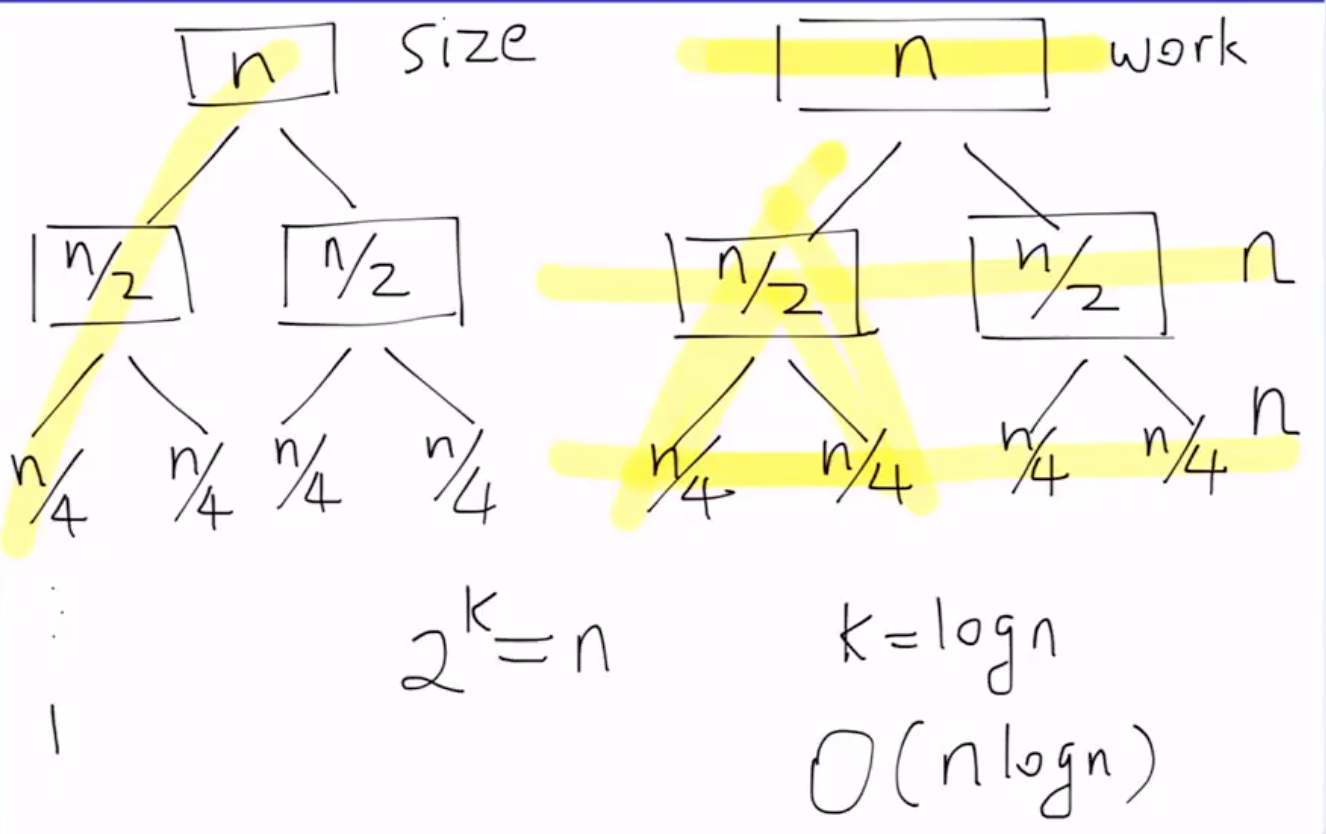
\includegraphics[width=\textwidth]{images/merge-sort-tree.png}
\end{itemize}

\end{document} 
